\lecture{ANOVA}{ANOVA}
\section{Analysis of Variance}

\title{Analysis of Variance}
\subtitle{Detecting a Difference Between Multiple Treatments}

%\author{Kelly Black}
%\institute{Clarkson University}
\date{14 November 2014}

\begin{frame}
  \titlepage
\end{frame}

\begin{frame}
  \frametitle{Outline}
  \tableofcontents[hideothersubsections,sectionstyle=show/hide]
\end{frame}



\subsection{Clicker Quiz}

\begin{frame}{Clicker Quiz}

  \iftoggle{clicker}{%

    The strength of three periodontal dressings is to be compared. The
    three different dressings are used on different patients, the
    strengths are measured. 

  \begin{columns}
    \column{.33\textwidth}
    \begin{tabular}{l}
      Coe \\ \hline
      546 kN/mm\\ 469 kN/mm\\ 602 kN/mm\\ 511 kN/mm\\ 665 kN/mm\\ 631
      kN/mm\\ 539 kN/mm\\ 631 kN/mm\\ 596 kN/mm\\ 546 kN/mm
    \end{tabular}
    \column{.33\textwidth}
    \begin{tabular}{l}
      Peripac \\ \hline
      91 kN/mm\\ 168 kN/mm\\ 168 kN/mm\\ 34 kN/mm\\ 71 kN/mm\\ 126 kN/mm\\
      77 kN/mm\\ 126 kN/mm\\ 119 kN/mm\\ 140 kN/mm
    \end{tabular}

    \column{.33\textwidth}
    \begin{tabular}{l}
      Putty \\ \hline
      631 kN/mm\\ 1058 kN/mm\\ 631 kN/mm\\ 882 kN/mm\\ 777 kN/mm\\
      1190 kN/mm\\ 833 kN/mm\\ 961 kN/mm\\ 785 kN/mm\\ 631 kN/mm
    \end{tabular}

  \end{columns}

    How do we treat these samples?


    \begin{tabular}{l@{\hspace{3em}}l@{\hspace{3em}}l@{\hspace{3em}}l}
      A: 2 Ind. Samples  & B: 2 Dep. Samples \\ 
      C: 3 Ind. Samples  & D: 3 Dep. Samples.
    \end{tabular}

    \vfill
    \vfill
    \vfill

  }

\end{frame}

\subsection{Example}

\begin{frame}{Comparing Multiple Independent Samples}

    The strength of three periodontal dressings is to be compared. The
    three different dressings are used on different patients, the
    strengths are measured. 

  \begin{columns}
    \column{.33\textwidth}
    \begin{tabular}{l}
      Coe \\ \hline
      546 kN/mm\\ 469 kN/mm\\ 602 kN/mm\\ 511 kN/mm\\ 665 kN/mm\\ 631
      kN/mm\\ 539 kN/mm\\ 631 kN/mm\\ 596 kN/mm\\ 546 kN/mm
    \end{tabular}
    \column{.33\textwidth}
    \begin{tabular}{l}
      Peripac \\ \hline
      91 kN/mm\\ 168 kN/mm\\ 168 kN/mm\\ 34 kN/mm\\ 71 kN/mm\\ 126 kN/mm\\
      77 kN/mm\\ 126 kN/mm\\ 119 kN/mm\\ 140 kN/mm
    \end{tabular}

    \column{.33\textwidth}
    \begin{tabular}{l}
      Putty \\ \hline
      631 kN/mm\\ 1058 kN/mm\\ 631 kN/mm\\ 882 kN/mm\\ 777 kN/mm\\
      1190 kN/mm\\ 833 kN/mm\\ 961 kN/mm\\ 785 kN/mm\\ 631 kN/mm
    \end{tabular}

  \end{columns}


\end{frame}


\begin{frame}{Comparing Multiple Independent Samples}

  The point estimates:
    \only<1>{%
      \redText{Coe}

      \begin{tabular}{rrrrr}
           Min. & 1st Qu. & Median  &  3rd Qu. &   Max. \\
           469.0   & 540.8 &   571.0  &  623.8 &   665.0 \\
      \end{tabular}

      \vfill

      \begin{tabular}{rr}
        Sample Mean & Sample Standard Deviation \\
        573.6 & 61.31
      \end{tabular}

      \vfill

      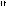
\includegraphics[width=4cm]{img/coePeriodontal}
      
    }
    \only<2>{%
      \redText{Peripac}

      \begin{tabular}{rrrrr}
           Min. & 1st Qu. & Median  &  3rd Qu. &   Max. \\
           34.0 &  80.5   & 122.5   &  136.5   & 168.0
      \end{tabular}

      \vfill

      \begin{tabular}{rr}
        Sample Mean & Sample Standard Deviation \\
        112 & 43.7
      \end{tabular}

      \vfill

      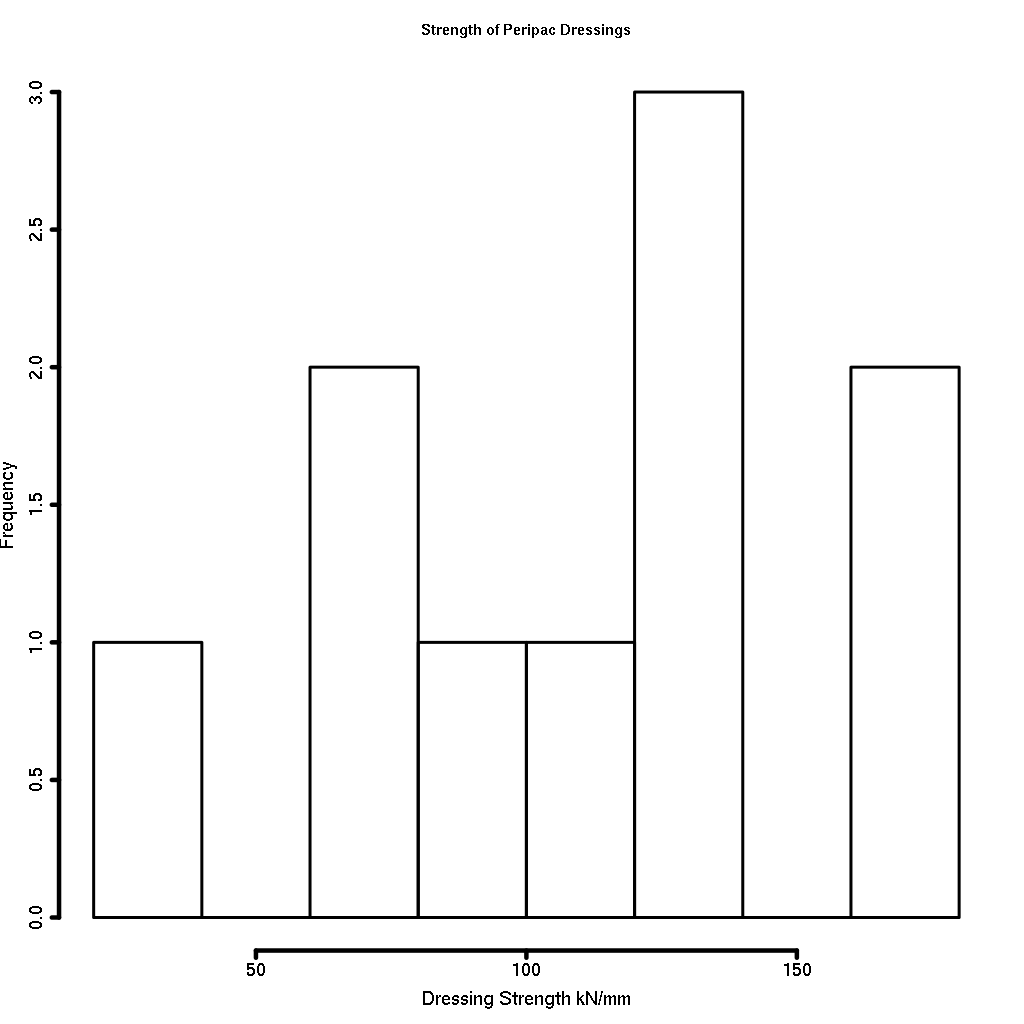
\includegraphics[width=4cm]{img/peripacPeriodontal.png}

    }
    \only<3>{%
      \redText{Putty}

      \begin{tabular}{rrrrr}
           Min. & 1st Qu. & Median  &  3rd Qu. &   Max. \\
           631.0&  667.5  & 809.0   &  941.2   & 1190.0
      \end{tabular}

      \vfill

      \begin{tabular}{rr}
        Sample Mean & Sample Standard Deviation \\
        837.9 & 189.9
      \end{tabular}

      \vfill

      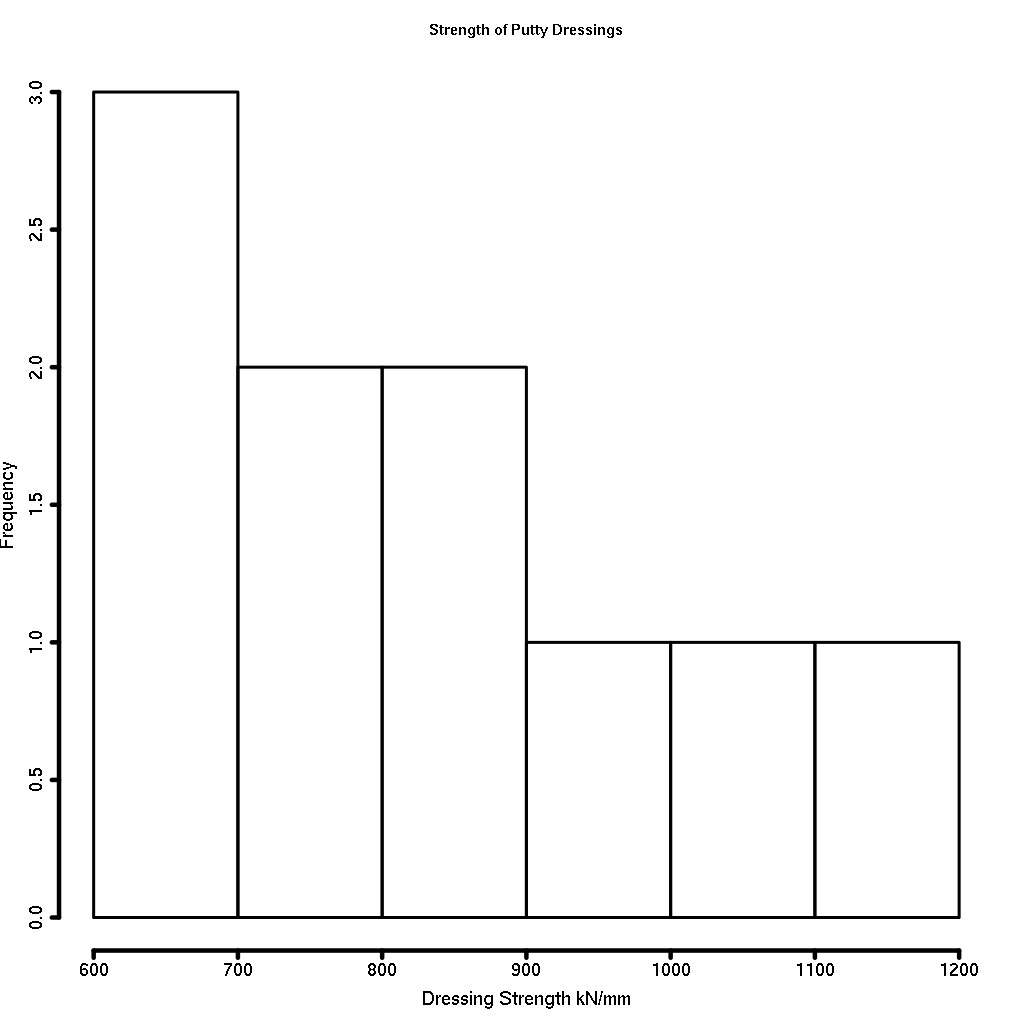
\includegraphics[width=4cm]{img/puttyPeriodontal}

    }



\end{frame}

\begin{frame}{Conclusions?}

  Is there a difference?

  \vfill

  \begin{columns}
    \column{.33\textwidth}

      \begin{tabular}{rr}
        $\bar{x}_1$ & $s_1$ \\
        573.6 & 61.31
      \end{tabular}


    \column{.33\textwidth}

      \begin{tabular}{rr}
        $\bar{x}_2$ & $s_2$ \\
        112 & 43.7
      \end{tabular}


    \column{.33\textwidth}

      \begin{tabular}{rr}
        $\bar{x}_3$ & $s_3$ \\
        837.9 & 189.9
      \end{tabular}


  \end{columns}

  \vfill

  \centerline{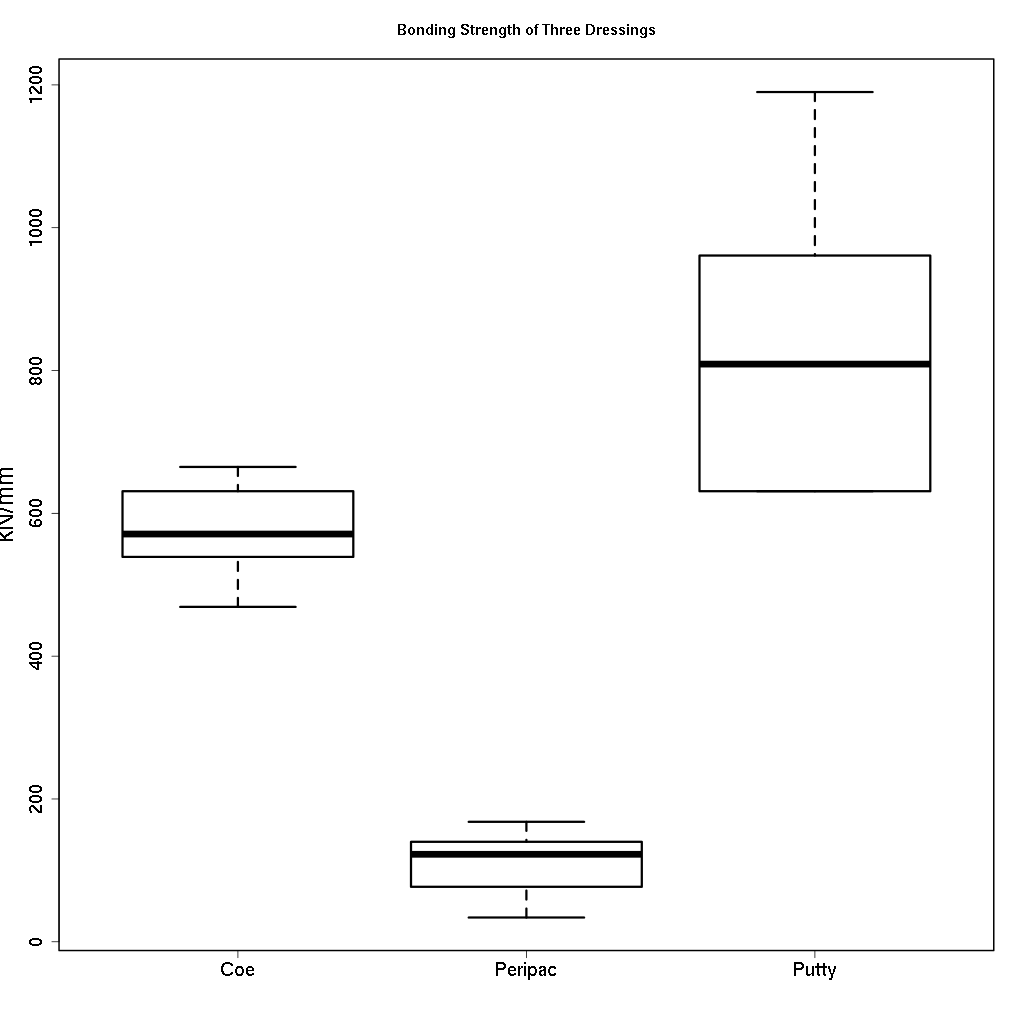
\includegraphics[width=4cm]{img/periodontalBoxplot}}

  \vfill

  How do we back up our claim?

  \vfill
  
\end{frame}

\subsection{Analysis of Variance}

\begin{frame}{Analysis of Variance}

  We have $k$ treatments and have measurements for each treatment. 


  \begin{eqnarray*}
    \begin{array}{llll@{\hspace{3em}}rr}
      x_{1,1}, & x_{1,2}, & \ldots & x_{1,n_1}, & \uncover<2->{ \bar{x_1} & n_1 } \\ 
      x_{2,1}, & x_{2,2}, & \ldots & x_{2,n_2}, & \uncover<2->{ \bar{x_2} & n_2 } \\
      \vdots  & \vdots  &       & \vdots \\
      x_{k,1}, & x_{k,2}, & \ldots & x_{k,n_k}. & \uncover<2->{ \bar{x_k} & n_k } 
    \end{array}
  \end{eqnarray*}

\end{frame}

\begin{frame}{Assumptions}

  \begin{eqnarray*}
    x_{i,j} & = & \mu_i + \sigma_{i,j}, \\
    \sigma_{i,j} & \thicksim & N(0,\sigma^2).
  \end{eqnarray*}

  \vfill

  We assume that all errors have the same variance!

  \vfill

  Hypothesis test:
  \begin{eqnarray*}
    H_0: & & \mu_1 = \mu_2 = \cdots = \mu_k, \\
    H_a: & & \mu_i \neq \mu_j ~\mathrm{for~some~}i,~j.
  \end{eqnarray*}

  \vfill
  
\end{frame}

\begin{frame}{Variance Away From What?}

  We have $k+1$ different point estimates for different means.
  \begin{eqnarray*}
    \bar{x}_1 & = & \frac{x_{1,1} + \cdots + x_{1,n_1}}{n_1}, \\
    \bar{x}_2 & = & \frac{x_{2,1} + \cdots + x_{2,n_2}}{n_2}, \\
              & \vdots & \\
    \bar{x}_k & = & \frac{x_{k,1} + \cdots + x_{k,n_k}}{n_k}, \\
    \bar{x}_T & = & \frac{n_1 \bar{x_1} + \cdots + n_k \bar{x_k}}{n_1+\cdots+n_k}.
  \end{eqnarray*}
  
\end{frame}

\begin{frame}{Three Measures of Variation}

  We have three measures of variance: \\
  \begin{tabular}{ll}
    SSTr & $=$ \\
    SSE  & $=$ \\
    SST  & $=$  
  \end{tabular}
  
\end{frame}

\begin{frame}{Interpretation}

  Hypothesis test:
  \begin{eqnarray*}
    H_0: & & \mu_1 = \mu_2 = \cdots = \mu_k, \\
    H_a: & & \mu_i \neq \mu_j ~\mathrm{for~some~}i,~j.
  \end{eqnarray*}

  \only<1>{\centerline{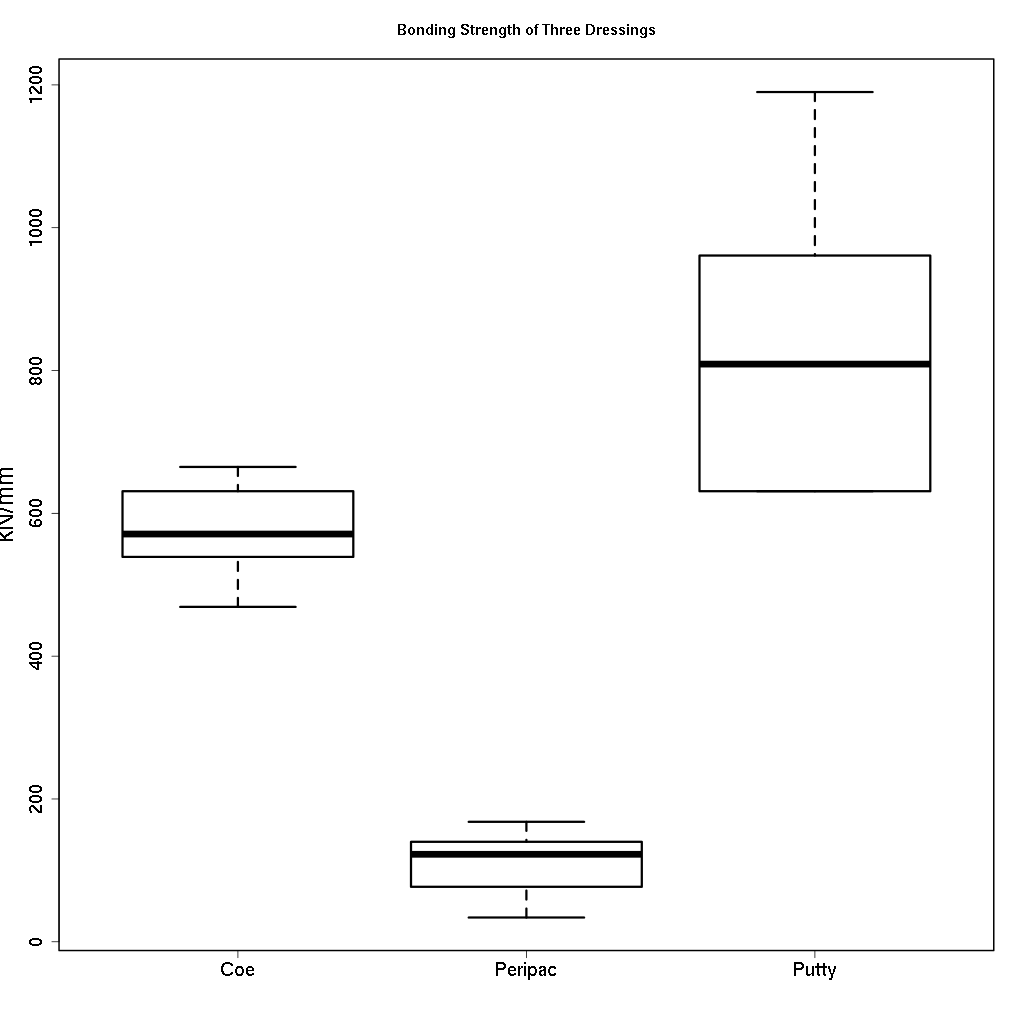
\includegraphics[width=4cm]{img/periodontalBoxplot}}}
  \only<2>{\centerline{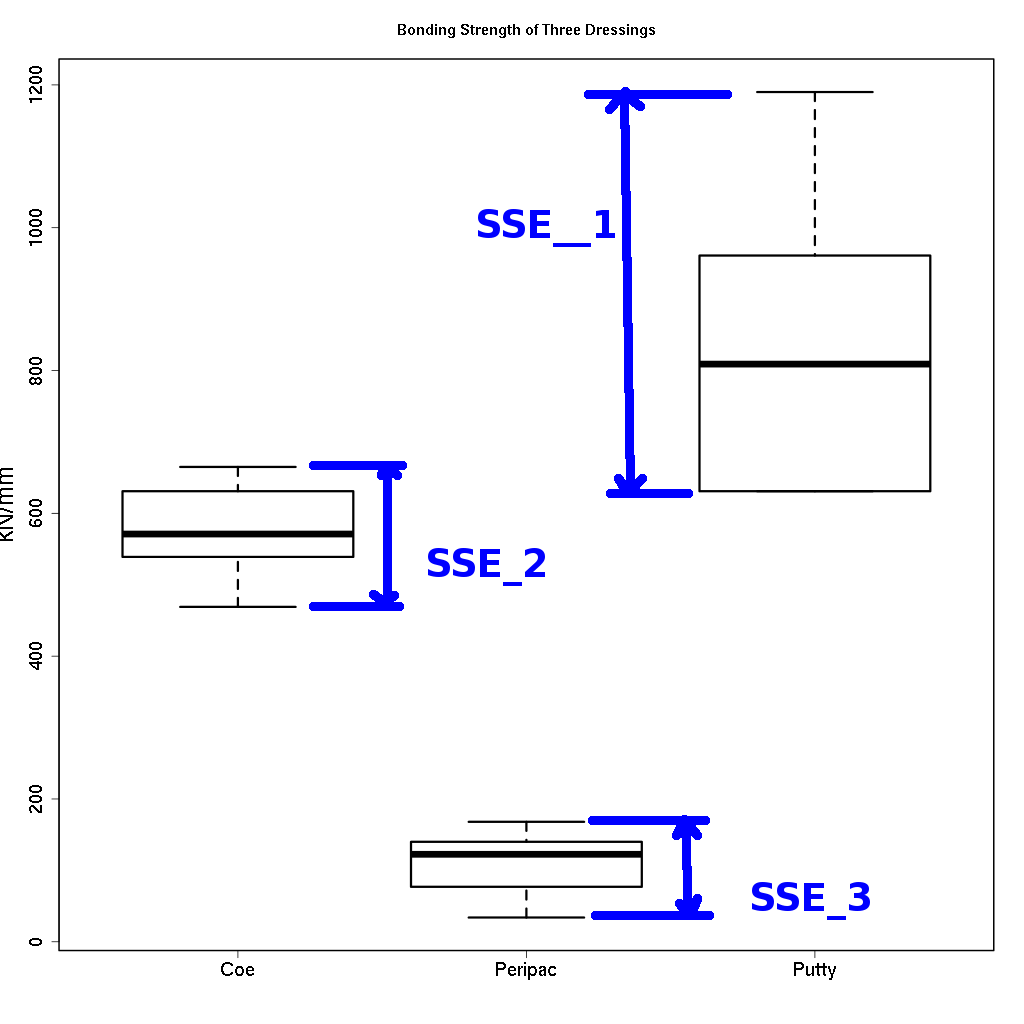
\includegraphics[width=4cm]{img/periodontalBoxplotSSE}}}
  \only<3>{\centerline{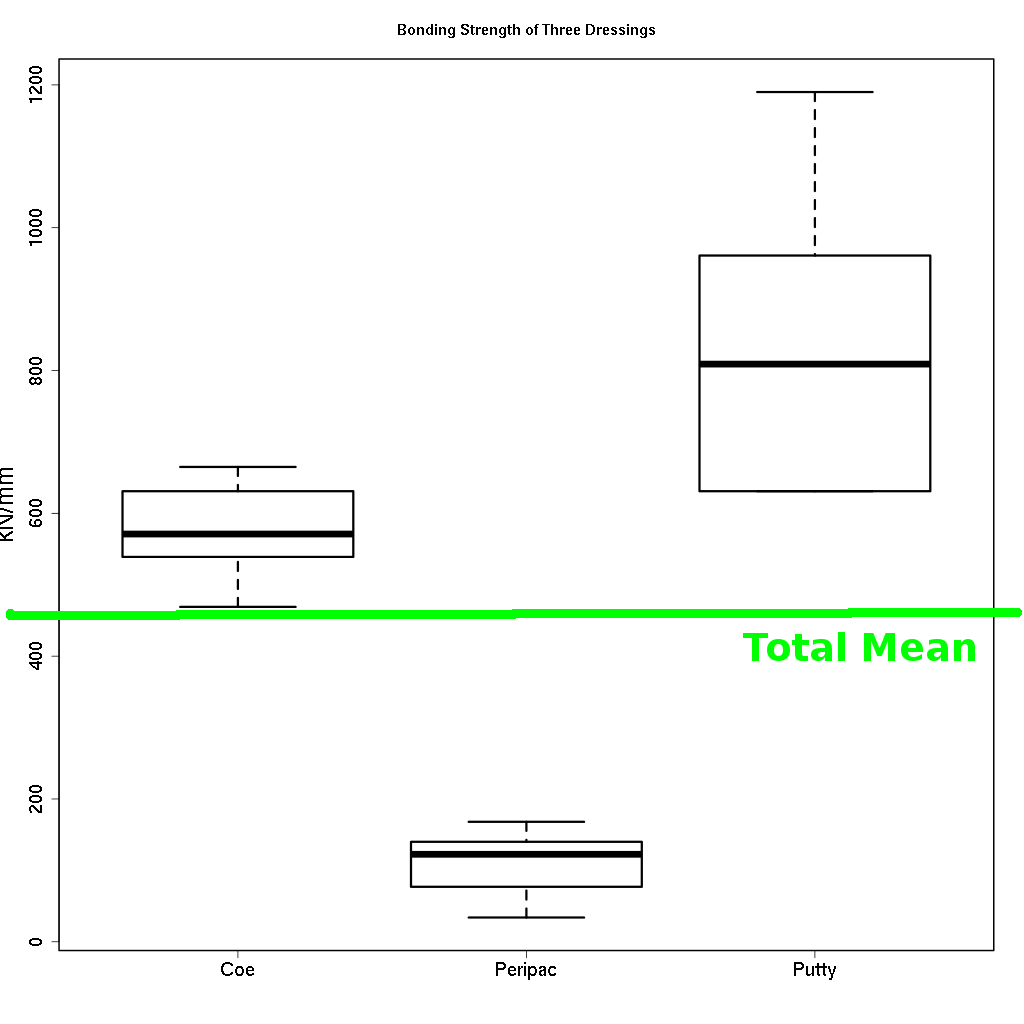
\includegraphics[width=4cm]{img/periodontalBoxplotTotalMean}}}
  \only<4>{\centerline{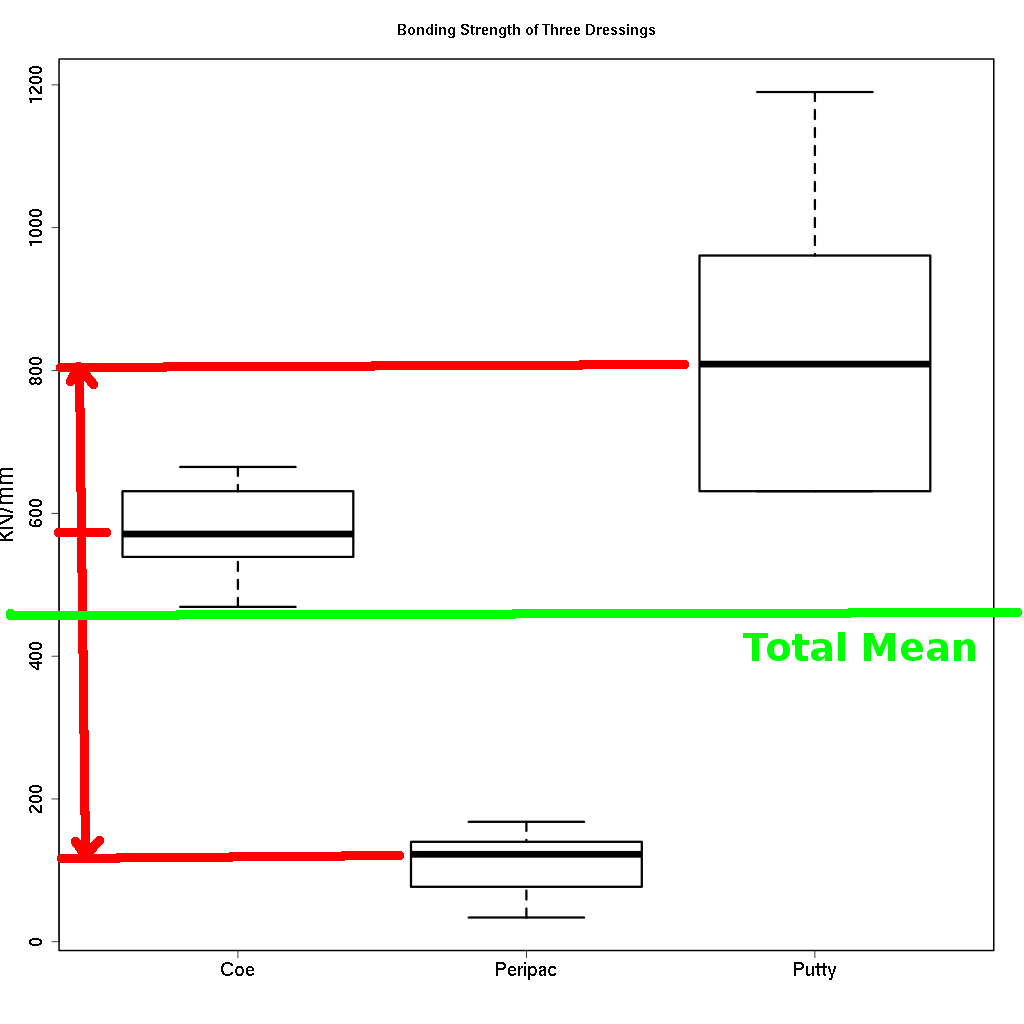
\includegraphics[width=4cm]{img/periodontalBoxplotSST}}}
  
\end{frame}

\begin{frame}{What Could Happen?}

  Assume the null hypothesis is true: \\
  \begin{tabular}{ll}
    SSTr small & SSE small \\
    SSTr small & SSE big \\
    SSTr big & SSE small \\
    SSTr big & SSE big \\
  \end{tabular}
  
\end{frame}

\begin{frame}{Bonding Strength for Periodontal Dressing}

  The strength of three periodontal dressings is to be compared. The
  three different dressings are used on different patients, the
  strengths are measured.

  \begin{columns}
    \column{.33\textwidth}
    \begin{tabular}{l}
      Coe \\ \hline
      546 kN/mm\\ 469 kN/mm\\ 602 kN/mm\\ 511 kN/mm\\ 665 kN/mm\\ 631
      kN/mm\\ 539 kN/mm\\ 631 kN/mm\\ 596 kN/mm\\ 546 kN/mm
    \end{tabular}
    \column{.33\textwidth}
    \begin{tabular}{l}
      Peripac \\ \hline
      91 kN/mm\\ 168 kN/mm\\ 168 kN/mm\\ 34 kN/mm\\ 71 kN/mm\\ 126 kN/mm\\
      77 kN/mm\\ 126 kN/mm\\ 119 kN/mm\\ 140 kN/mm
    \end{tabular}

    \column{.33\textwidth}
    \begin{tabular}{l}
      Putty \\ \hline
      631 kN/mm\\ 1058 kN/mm\\ 631 kN/mm\\ 882 kN/mm\\ 777 kN/mm\\
      1190 kN/mm\\ 833 kN/mm\\ 961 kN/mm\\ 785 kN/mm\\ 631 kN/mm
    \end{tabular}

  \end{columns}

\end{frame}

\begin{frame}{Bonding Strength for Periodontal Dressing}

  The strength of three periodontal dressings is to be compared. The
  three different dressings are used on different patients, the
  strengths are measured.

  The three measures of variance: \\
  \begin{tabular}{ll}
    SSTr & $=$ \\
    SSE  & $=$ \\
    SST  & $=$  
  \end{tabular}


\end{frame}

\begin{frame}{The F Distribution}

  \begin{columns}
    \column{.5\textwidth}

    We define the following quantities:
    \begin{eqnarray*}
      MSTR & = & \frac{SSTr}{k-1}, \\
      MSE  & = & \frac{SSE}{N_T - k}, \\
      F    & = & \frac{MSTR}{MSE}.
    \end{eqnarray*}

  \vfill

    \column{.5\textwidth}

    \vfill

    \centerline{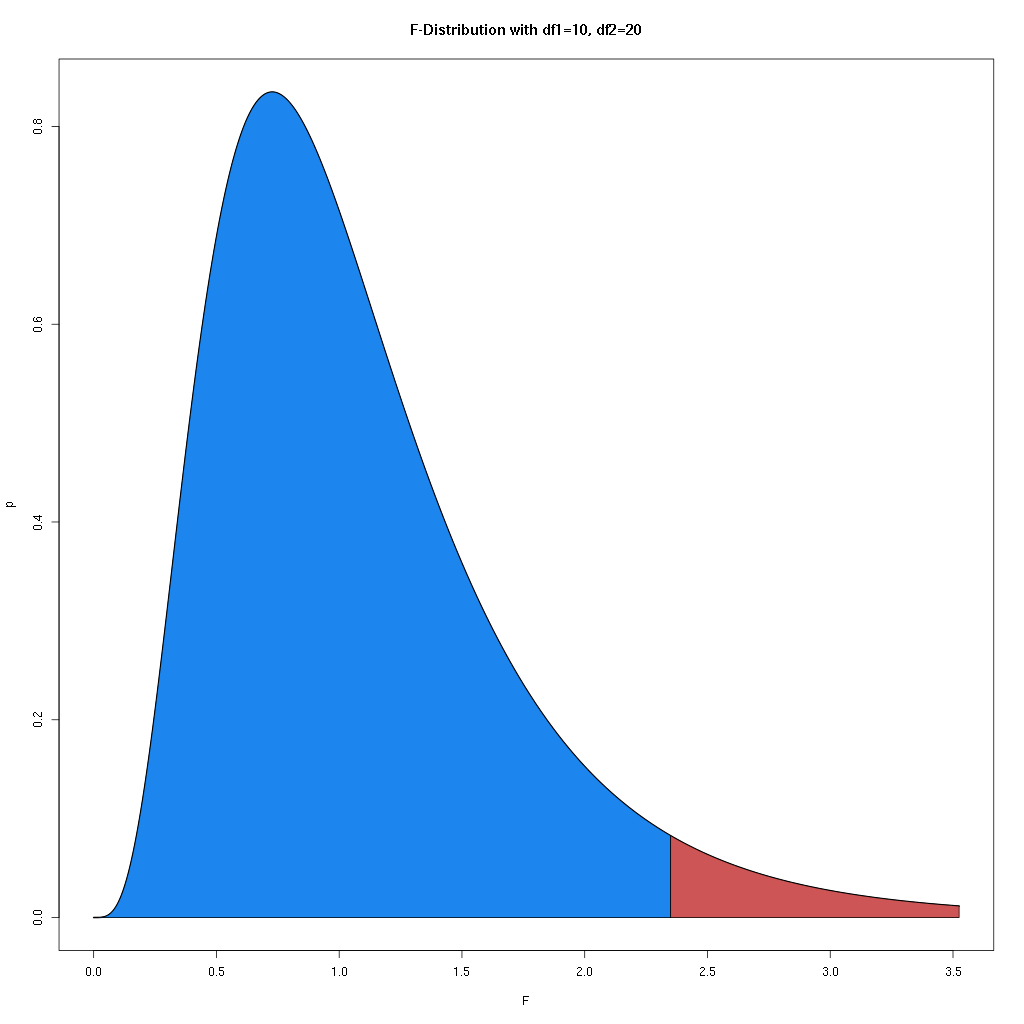
\includegraphics[width=4cm]{img/FDistribution}}

    \vfill

    \end{columns}
  
\end{frame}


\definecolor{light-gray}{gray}{0.7} 

\begin{frame}{F-Tables}
{\small Approximation of the critical values for the $F$-distribution for $\alpha=0.1$. }
 {
   \fontencoding{T1}
   \fontfamily{pcr}
   \fontseries{m}
   \fontshape{n}
   \fontsize{5pt}{5pt}
   \selectfont
   \begin{tabular}{l|lllllllllllll} 
     df2  & df1      1  &      2  &      3  &      4  &      5  &      6  &      7  &      8  &      9   \\ 
     1 & 39.8635 & 49.5000 & 53.5932 & 55.8330 & 57.2401 & 58.2044 & 58.9060 & 59.4390 & 59.8576   \\[5pt] \arrayrulecolor{light-gray}\hline\arrayrulecolor{black}  
     2 & 8.5263 & 9.0000 & 9.1618 & 9.2434 & 9.2926 & 9.3255 & 9.3491 & 9.3668 & 9.3805  \\[5pt] \arrayrulecolor{light-gray}\hline\arrayrulecolor{black}  
     3 & 5.5383 & 5.4624 & 5.3908 & 5.3426 & 5.3092 & 5.2847 & 5.2662 & 5.2517 & 5.2400  \\[5pt] \arrayrulecolor{light-gray}\hline\arrayrulecolor{black}  
     4 & 4.5448 & 4.3246 & 4.1909 & 4.1072 & 4.0506 & 4.0097 & 3.9790 & 3.9549 & 3.9357  \\[5pt] \arrayrulecolor{light-gray}\hline\arrayrulecolor{black}  
     5 & 4.0604 & 3.7797 & 3.6195 & 3.5202 & 3.4530 & 3.4045 & 3.3679 & 3.3393 & 3.3163  \\[5pt] \arrayrulecolor{light-gray}\hline\arrayrulecolor{black}  
     \\ 
     6 & 3.7759 & 3.4633 & 3.2888 & 3.1808 & 3.1075 & 3.0546 & 3.0145 & 2.9830 & 2.9577  \\[5pt] \arrayrulecolor{light-gray}\hline\arrayrulecolor{black}  
     7 & 3.5894 & 3.2574 & 3.0741 & 2.9605 & 2.8833 & 2.8274 & 2.7849 & 2.7516 & 2.7247  \\[5pt] \arrayrulecolor{light-gray}\hline\arrayrulecolor{black}  
     8 & 3.4579 & 3.1131 & 2.9238 & 2.8064 & 2.7264 & 2.6683 & 2.6241 & 2.5893 & 2.5612  \\[5pt] \arrayrulecolor{light-gray}\hline\arrayrulecolor{black}  
     9 & 3.3603 & 3.0065 & 2.8129 & 2.6927 & 2.6106 & 2.5509 & 2.5053 & 2.4694 & 2.4403  \\[5pt] \arrayrulecolor{light-gray}\hline\arrayrulecolor{black}  
     10 & 3.2850 & 2.9245 & 2.7277 & 2.6053 & 2.5216 & 2.4606 & 2.4140 & 2.3772 & 2.3473  \\[5pt] \arrayrulecolor{light-gray}\hline\arrayrulecolor{black}  
     \\ 
     11 & 3.2252 & 2.8595 & 2.6602 & 2.5362 & 2.4512 & 2.3891 & 2.3416 & 2.3040 & 2.2735  \\[5pt] \arrayrulecolor{light-gray}\hline\arrayrulecolor{black}  
     12 & 3.1765 & 2.8068 & 2.6055 & 2.4801 & 2.3940 & 2.3310 & 2.2828 & 2.2446 & 2.2135  \\[5pt] \arrayrulecolor{light-gray}\hline\arrayrulecolor{black}  
     13 & 3.1362 & 2.7632 & 2.5603 & 2.4337 & 2.3467 & 2.2830 & 2.2341 & 2.1953 & 2.1638  \\[5pt] \arrayrulecolor{light-gray}\hline\arrayrulecolor{black}  
     14 & 3.1022 & 2.7265 & 2.5222 & 2.3947 & 2.3069 & 2.2426 & 2.1931 & 2.1539 & 2.1220  \\[5pt] \arrayrulecolor{light-gray}\hline\arrayrulecolor{black}  
     15 & 3.0732 & 2.6952 & 2.4898 & 2.3614 & 2.2730 & 2.2081 & 2.1582 & 2.1185 & 2.0862  \\[5pt] \arrayrulecolor{light-gray}\hline\arrayrulecolor{black}  
     \\ 
     16 & 3.0481 & 2.6682 & 2.4618 & 2.3327 & 2.2438 & 2.1783 & 2.1280 & 2.0880 & 2.0553  \\[5pt] \arrayrulecolor{light-gray}\hline\arrayrulecolor{black}  
     17 & 3.0262 & 2.6446 & 2.4374 & 2.3077 & 2.2183 & 2.1524 & 2.1017 & 2.0613 & 2.0284  \\[5pt] \arrayrulecolor{light-gray}\hline\arrayrulecolor{black}  
     18 & 3.0070 & 2.6239 & 2.4160 & 2.2858 & 2.1958 & 2.1296 & 2.0785 & 2.0379 & 2.0047  \\[5pt] \arrayrulecolor{light-gray}\hline\arrayrulecolor{black}  
     19 & 2.9899 & 2.6056 & 2.3970 & 2.2663 & 2.1760 & 2.1094 & 2.0580 & 2.0171 & 1.9836  \\[5pt] \arrayrulecolor{light-gray}\hline\arrayrulecolor{black}  
     20 & 2.9747 & 2.5893 & 2.3801 & 2.2489 & 2.1582 & 2.0913 & 2.0397 & 1.9985 & 1.9649  \\[5pt] \arrayrulecolor{light-gray}\hline\arrayrulecolor{black}  
   \end{tabular}
}
  
\end{frame}


\begin{frame}{\small Find the critical F for df1=6, df2=8, $\alpha=0.1$}
{\small Approximation of the critical values for the $F$-distribution for $\alpha=0.1$. }
 {
   \fontencoding{T1}
   \fontfamily{pcr}
   \fontseries{m}
   \fontshape{n}
   \fontsize{5pt}{5pt}
   \selectfont
   \begin{tabular}{l|lllllllll} 
     df2  & df1      1  &      2  &      3  &      4  &      5  &      6  &      7  &      8  &      9   \\ 
     1 & 39.8635 & 49.5000 & 53.5932 & 55.8330 & 57.2401 & 58.2044 & 58.9060 & 59.4390 & 59.8576   \\[5pt] \arrayrulecolor{light-gray}\hline\arrayrulecolor{black}  
     2 & 8.5263 & 9.0000 & 9.1618 & 9.2434 & 9.2926 & 9.3255 & 9.3491 & 9.3668 & 9.3805  \\[5pt] \arrayrulecolor{light-gray}\hline\arrayrulecolor{black}  
     3 & 5.5383 & 5.4624 & 5.3908 & 5.3426 & 5.3092 & 5.2847 & 5.2662 & 5.2517 & 5.2400  \\[5pt] \arrayrulecolor{light-gray}\hline\arrayrulecolor{black}  
     4 & 4.5448 & 4.3246 & 4.1909 & 4.1072 & 4.0506 & 4.0097 & 3.9790 & 3.9549 & 3.9357  \\[5pt] \arrayrulecolor{light-gray}\hline\arrayrulecolor{black}  
     5 & 4.0604 & 3.7797 & 3.6195 & 3.5202 & 3.4530 & 3.4045 & 3.3679 & 3.3393 & 3.3163  \\[5pt] \arrayrulecolor{light-gray}\hline\arrayrulecolor{black}  
     \\ 
     6 & 3.7759 & 3.4633 & 3.2888 & 3.1808 & 3.1075 & 3.0546 & 3.0145 & 2.9830 & 2.9577  \\[5pt] \arrayrulecolor{light-gray}\hline\arrayrulecolor{black}  
     7 & 3.5894 & 3.2574 & 3.0741 & 2.9605 & 2.8833 & 2.8274 & 2.7849 & 2.7516 & 2.7247  \\[5pt] \arrayrulecolor{light-gray}\hline\arrayrulecolor{black}  
     8 & 3.4579 & 3.1131 & 2.9238 & 2.8064 & 2.7264 & 2.6683 & 2.6241 & 2.5893 & 2.5612  \\[5pt] \arrayrulecolor{light-gray}\hline\arrayrulecolor{black}  
     9 & 3.3603 & 3.0065 & 2.8129 & 2.6927 & 2.6106 & 2.5509 & 2.5053 & 2.4694 & 2.4403  \\[5pt] \arrayrulecolor{light-gray}\hline\arrayrulecolor{black}  
     10 & 3.2850 & 2.9245 & 2.7277 & 2.6053 & 2.5216 & 2.4606 & 2.4140 & 2.3772 & 2.3473  \\[5pt] \arrayrulecolor{light-gray}\hline\arrayrulecolor{black}  
     \\ 
     11 & 3.2252 & 2.8595 & 2.6602 & 2.5362 & 2.4512 & 2.3891 & 2.3416 & 2.3040 & 2.2735  \\[5pt] \arrayrulecolor{light-gray}\hline\arrayrulecolor{black}  
     12 & 3.1765 & 2.8068 & 2.6055 & 2.4801 & 2.3940 & 2.3310 & 2.2828 & 2.2446 & 2.2135  \\[5pt] \arrayrulecolor{light-gray}\hline\arrayrulecolor{black}  
     13 & 3.1362 & 2.7632 & 2.5603 & 2.4337 & 2.3467 & 2.2830 & 2.2341 & 2.1953 & 2.1638  \\[5pt] \arrayrulecolor{light-gray}\hline\arrayrulecolor{black}  
     14 & 3.1022 & 2.7265 & 2.5222 & 2.3947 & 2.3069 & 2.2426 & 2.1931 & 2.1539 & 2.1220  \\[5pt] \arrayrulecolor{light-gray}\hline\arrayrulecolor{black}  
     15 & 3.0732 & 2.6952 & 2.4898 & 2.3614 & 2.2730 & 2.2081 & 2.1582 & 2.1185 & 2.0862  \\[5pt] \arrayrulecolor{light-gray}\hline\arrayrulecolor{black}  
     \\ 
     16 & 3.0481 & 2.6682 & 2.4618 & 2.3327 & 2.2438 & 2.1783 & 2.1280 & 2.0880 & 2.0553  \\[5pt] \arrayrulecolor{light-gray}\hline\arrayrulecolor{black}  
     17 & 3.0262 & 2.6446 & 2.4374 & 2.3077 & 2.2183 & 2.1524 & 2.1017 & 2.0613 & 2.0284  \\[5pt] \arrayrulecolor{light-gray}\hline\arrayrulecolor{black}  
     18 & 3.0070 & 2.6239 & 2.4160 & 2.2858 & 2.1958 & 2.1296 & 2.0785 & 2.0379 & 2.0047  \\[5pt] \arrayrulecolor{light-gray}\hline\arrayrulecolor{black}  
     19 & 2.9899 & 2.6056 & 2.3970 & 2.2663 & 2.1760 & 2.1094 & 2.0580 & 2.0171 & 1.9836  \\[5pt] \arrayrulecolor{light-gray}\hline\arrayrulecolor{black}  
     20 & 2.9747 & 2.5893 & 2.3801 & 2.2489 & 2.1582 & 2.0913 & 2.0397 & 1.9985 & 1.9649  \\[5pt] \arrayrulecolor{light-gray}\hline\arrayrulecolor{black}  
   \end{tabular}
}
  
\end{frame}


\begin{frame}{\small Find the critical F for df1=6, df2=8, $\alpha=0.1$}
{\small Approximation of the critical values for the $F$-distribution for $\alpha=0.1$. }
 {
   \fontencoding{T1}
   \fontfamily{pcr}
   \fontseries{m}
   \fontshape{n}
   \fontsize{5pt}{5pt}
   \selectfont
   \begin{tabular}{l|lllll>{\columncolor{light-blue}}llll} 
     df2  & df1      1  &      2  &      3  &      4  &      5  &      6  &      7  &      8  &      9   \\ 
     1 & 39.8635 & 49.5000 & 53.5932 & 55.8330 & 57.2401 & 58.2044 & 58.9060 & 59.4390 & 59.8576   \\[5pt] \arrayrulecolor{light-gray}\hline\arrayrulecolor{black}  
     2 & 8.5263 & 9.0000 & 9.1618 & 9.2434 & 9.2926 & 9.3255 & 9.3491 & 9.3668 & 9.3805  \\[5pt] \arrayrulecolor{light-gray}\hline\arrayrulecolor{black}  
     3 & 5.5383 & 5.4624 & 5.3908 & 5.3426 & 5.3092 & 5.2847 & 5.2662 & 5.2517 & 5.2400  \\[5pt] \arrayrulecolor{light-gray}\hline\arrayrulecolor{black}  
     4 & 4.5448 & 4.3246 & 4.1909 & 4.1072 & 4.0506 & 4.0097 & 3.9790 & 3.9549 & 3.9357  \\[5pt] \arrayrulecolor{light-gray}\hline\arrayrulecolor{black}  
     5 & 4.0604 & 3.7797 & 3.6195 & 3.5202 & 3.4530 & 3.4045 & 3.3679 & 3.3393 & 3.3163  \\[5pt] \arrayrulecolor{light-gray}\hline\arrayrulecolor{black}  
     \\ 
     6 & 3.7759 & 3.4633 & 3.2888 & 3.1808 & 3.1075 & 3.0546 & 3.0145 & 2.9830 & 2.9577  \\[5pt] \arrayrulecolor{light-gray}\hline\arrayrulecolor{black}  
     7 & 3.5894 & 3.2574 & 3.0741 & 2.9605 & 2.8833 & 2.8274 & 2.7849 & 2.7516 & 2.7247  \\[5pt] \arrayrulecolor{light-gray}\hline\arrayrulecolor{black}  
     8 & 3.4579 & 3.1131 & 2.9238 & 2.8064 & 2.7264 & 2.6683 & 2.6241 & 2.5893 & 2.5612  \\[5pt] \arrayrulecolor{light-gray}\hline\arrayrulecolor{black}  
     9 & 3.3603 & 3.0065 & 2.8129 & 2.6927 & 2.6106 & 2.5509 & 2.5053 & 2.4694 & 2.4403  \\[5pt] \arrayrulecolor{light-gray}\hline\arrayrulecolor{black}  
     10 & 3.2850 & 2.9245 & 2.7277 & 2.6053 & 2.5216 & 2.4606 & 2.4140 & 2.3772 & 2.3473  \\[5pt] \arrayrulecolor{light-gray}\hline\arrayrulecolor{black}  
     \\ 
     11 & 3.2252 & 2.8595 & 2.6602 & 2.5362 & 2.4512 & 2.3891 & 2.3416 & 2.3040 & 2.2735  \\[5pt] \arrayrulecolor{light-gray}\hline\arrayrulecolor{black}  
     12 & 3.1765 & 2.8068 & 2.6055 & 2.4801 & 2.3940 & 2.3310 & 2.2828 & 2.2446 & 2.2135  \\[5pt] \arrayrulecolor{light-gray}\hline\arrayrulecolor{black}  
     13 & 3.1362 & 2.7632 & 2.5603 & 2.4337 & 2.3467 & 2.2830 & 2.2341 & 2.1953 & 2.1638  \\[5pt] \arrayrulecolor{light-gray}\hline\arrayrulecolor{black}  
     14 & 3.1022 & 2.7265 & 2.5222 & 2.3947 & 2.3069 & 2.2426 & 2.1931 & 2.1539 & 2.1220  \\[5pt] \arrayrulecolor{light-gray}\hline\arrayrulecolor{black}  
     15 & 3.0732 & 2.6952 & 2.4898 & 2.3614 & 2.2730 & 2.2081 & 2.1582 & 2.1185 & 2.0862  \\[5pt] \arrayrulecolor{light-gray}\hline\arrayrulecolor{black}  
     \\ 
     16 & 3.0481 & 2.6682 & 2.4618 & 2.3327 & 2.2438 & 2.1783 & 2.1280 & 2.0880 & 2.0553  \\[5pt] \arrayrulecolor{light-gray}\hline\arrayrulecolor{black}  
     17 & 3.0262 & 2.6446 & 2.4374 & 2.3077 & 2.2183 & 2.1524 & 2.1017 & 2.0613 & 2.0284  \\[5pt] \arrayrulecolor{light-gray}\hline\arrayrulecolor{black}  
     18 & 3.0070 & 2.6239 & 2.4160 & 2.2858 & 2.1958 & 2.1296 & 2.0785 & 2.0379 & 2.0047  \\[5pt] \arrayrulecolor{light-gray}\hline\arrayrulecolor{black}  
     19 & 2.9899 & 2.6056 & 2.3970 & 2.2663 & 2.1760 & 2.1094 & 2.0580 & 2.0171 & 1.9836  \\[5pt] \arrayrulecolor{light-gray}\hline\arrayrulecolor{black}  
     20 & 2.9747 & 2.5893 & 2.3801 & 2.2489 & 2.1582 & 2.0913 & 2.0397 & 1.9985 & 1.9649  \\[5pt] \arrayrulecolor{light-gray}\hline\arrayrulecolor{black}  
   \end{tabular}
}
  
\end{frame}

\begin{frame}{\small Find the critical F for df1=6, df2=8, $\alpha=0.1$}
{\small Approximation of the critical values for the $F$-distribution for $\alpha=0.1$. }
 {
   \fontencoding{T1}
   \fontfamily{pcr}
   \fontseries{m}
   \fontshape{n}
   \fontsize{5pt}{5pt}
   \selectfont
   \begin{tabular}{l|lllll>{\columncolor{light-blue}}llll} 
     df2  & df1      1  &      2  &      3  &      4  &      5  &      6  &      7  &      8  &      9   \\ 
     1 & 39.8635 & 49.5000 & 53.5932 & 55.8330 & 57.2401 & 58.2044 & 58.9060 & 59.4390 & 59.8576   \\[5pt] \arrayrulecolor{light-gray}\hline\arrayrulecolor{black}  
     2 & 8.5263 & 9.0000 & 9.1618 & 9.2434 & 9.2926 & 9.3255 & 9.3491 & 9.3668 & 9.3805  \\[5pt] \arrayrulecolor{light-gray}\hline\arrayrulecolor{black}  
     3 & 5.5383 & 5.4624 & 5.3908 & 5.3426 & 5.3092 & 5.2847 & 5.2662 & 5.2517 & 5.2400  \\[5pt] \arrayrulecolor{light-gray}\hline\arrayrulecolor{black}  
     4 & 4.5448 & 4.3246 & 4.1909 & 4.1072 & 4.0506 & 4.0097 & 3.9790 & 3.9549 & 3.9357  \\[5pt] \arrayrulecolor{light-gray}\hline\arrayrulecolor{black}  
     5 & 4.0604 & 3.7797 & 3.6195 & 3.5202 & 3.4530 & 3.4045 & 3.3679 & 3.3393 & 3.3163  \\[5pt] \arrayrulecolor{light-gray}\hline\arrayrulecolor{black}  
     \\ 
     6 & 3.7759 & 3.4633 & 3.2888 & 3.1808 & 3.1075 & 3.0546 & 3.0145 & 2.9830 & 2.9577  \\[5pt] \arrayrulecolor{light-gray}\hline\arrayrulecolor{black}  
     7 & 3.5894 & 3.2574 & 3.0741 & 2.9605 & 2.8833 & 2.8274 & 2.7849 & 2.7516 & 2.7247  \\[5pt] \arrayrulecolor{light-gray}\hline\arrayrulecolor{black}  
\rowcolor{light-red} 8 & 3.4579 & 3.1131 & 2.9238 & 2.8064 & 2.7264 & 2.6683 & 2.6241 & 2.5893 & 2.5612  \\[5pt] \arrayrulecolor{light-gray}\hline\arrayrulecolor{black}  
     9 & 3.3603 & 3.0065 & 2.8129 & 2.6927 & 2.6106 & 2.5509 & 2.5053 & 2.4694 & 2.4403  \\[5pt] \arrayrulecolor{light-gray}\hline\arrayrulecolor{black}  
     10 & 3.2850 & 2.9245 & 2.7277 & 2.6053 & 2.5216 & 2.4606 & 2.4140 & 2.3772 & 2.3473  \\[5pt] \arrayrulecolor{light-gray}\hline\arrayrulecolor{black}  
     \\ 
     11 & 3.2252 & 2.8595 & 2.6602 & 2.5362 & 2.4512 & 2.3891 & 2.3416 & 2.3040 & 2.2735  \\[5pt] \arrayrulecolor{light-gray}\hline\arrayrulecolor{black}  
     12 & 3.1765 & 2.8068 & 2.6055 & 2.4801 & 2.3940 & 2.3310 & 2.2828 & 2.2446 & 2.2135  \\[5pt] \arrayrulecolor{light-gray}\hline\arrayrulecolor{black}  
     13 & 3.1362 & 2.7632 & 2.5603 & 2.4337 & 2.3467 & 2.2830 & 2.2341 & 2.1953 & 2.1638  \\[5pt] \arrayrulecolor{light-gray}\hline\arrayrulecolor{black}  
     14 & 3.1022 & 2.7265 & 2.5222 & 2.3947 & 2.3069 & 2.2426 & 2.1931 & 2.1539 & 2.1220  \\[5pt] \arrayrulecolor{light-gray}\hline\arrayrulecolor{black}  
     15 & 3.0732 & 2.6952 & 2.4898 & 2.3614 & 2.2730 & 2.2081 & 2.1582 & 2.1185 & 2.0862  \\[5pt] \arrayrulecolor{light-gray}\hline\arrayrulecolor{black}  
     \\ 
     16 & 3.0481 & 2.6682 & 2.4618 & 2.3327 & 2.2438 & 2.1783 & 2.1280 & 2.0880 & 2.0553  \\[5pt] \arrayrulecolor{light-gray}\hline\arrayrulecolor{black}  
     17 & 3.0262 & 2.6446 & 2.4374 & 2.3077 & 2.2183 & 2.1524 & 2.1017 & 2.0613 & 2.0284  \\[5pt] \arrayrulecolor{light-gray}\hline\arrayrulecolor{black}  
     18 & 3.0070 & 2.6239 & 2.4160 & 2.2858 & 2.1958 & 2.1296 & 2.0785 & 2.0379 & 2.0047  \\[5pt] \arrayrulecolor{light-gray}\hline\arrayrulecolor{black}  
     19 & 2.9899 & 2.6056 & 2.3970 & 2.2663 & 2.1760 & 2.1094 & 2.0580 & 2.0171 & 1.9836  \\[5pt] \arrayrulecolor{light-gray}\hline\arrayrulecolor{black}  
     20 & 2.9747 & 2.5893 & 2.3801 & 2.2489 & 2.1582 & 2.0913 & 2.0397 & 1.9985 & 1.9649  \\[5pt] \arrayrulecolor{light-gray}\hline\arrayrulecolor{black}  
   \end{tabular}
}
  
\end{frame}


\begin{frame}{The F Statistic for the Strength of Three Periodontal Dressings }

  \begin{columns}
    \column{.5\textwidth}

    We define the following quantities:
    \begin{eqnarray*}
      MSTR & = & \frac{SSTr}{k-1}, \\
      MSE  & = & \frac{SSE}{N_T - k}, \\
      F*   & = & \frac{MSTR}{MSE}, \\
      F_{cr} & = &
    \end{eqnarray*}

    \vfill

    \column{.5\textwidth}

    \vfill

    \centerline{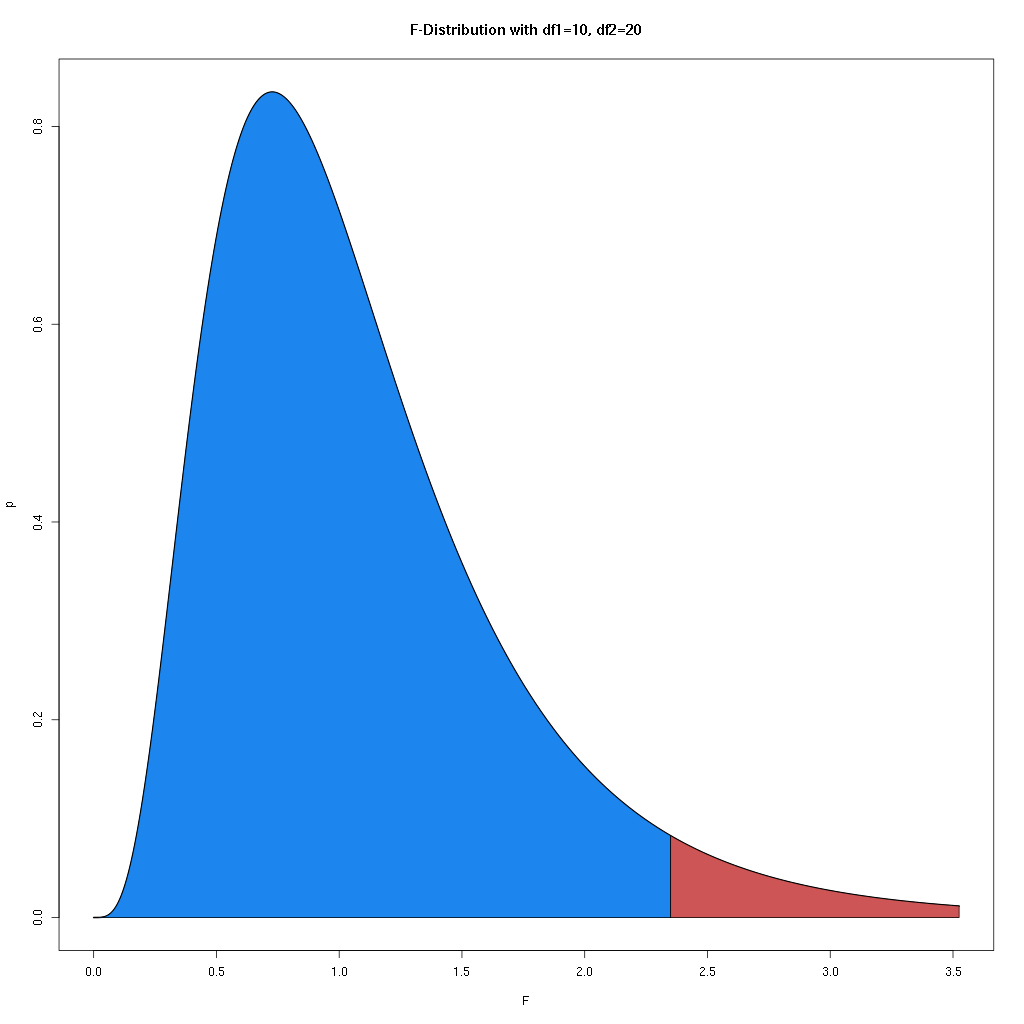
\includegraphics[width=4cm]{img/FDistribution}}

    \vfill

    \end{columns}

    \uncover<2->{%

      We can reject $H_0$ with a confidence level of 95\% and using an F distribution with df1=2 and df2=27.

    }
  
\end{frame}



%%% Local Variables: 
%%% mode: latex
%%% TeX-master: t
%%% End: 
